%%%%%%%%%%%%%%%%%%%%%%%%%%%%% Define Article %%%%%%%%%%%%%%%%%%%%%%%%%%%%%%%%%%
\documentclass{article}
%%%%%%%%%%%%%%%%%%%%%%%%%%%%%%%%%%%%%%%%%%%%%%%%%%%%%%%%%%%%%%%%%%%%%%%%%%%%%%%

%%%%%%%%%%%%%%%%%%%%%%%%%%%%% Using Packages %%%%%%%%%%%%%%%%%%%%%%%%%%%%%%%%%%
\usepackage{geometry}
\usepackage{graphicx}
\usepackage{amssymb}
\usepackage{amsmath}
\usepackage{amsthm}
\usepackage{empheq}
\usepackage{mdframed}
\usepackage{booktabs}
\usepackage{lipsum}
\usepackage{graphicx}
\usepackage{color}
\usepackage{psfrag}
\usepackage{pgfplots}
\usepackage{bm}
\usepackage{hyperref}
\hypersetup{
  colorlinks,
  citecolor=black,
  filecolor=black,
  linkcolor=black,
  urlcolor=black
}

\usepackage{fontawesome5}
\usepackage{todonotes}
%%%%%%%%%%%%%%%%%%%%%%%%%%%%%%%%%%%%%%%%%%%%%%%%%%%%%%%%%%%%%%%%%%%%%%%%%%%%%%%

% Other Settings

%%%%%%%%%%%%%%%%%%%%%%%%%% Page Setting %%%%%%%%%%%%%%%%%%%%%%%%%%%%%%%%%%%%%%%
\geometry{a4paper}

%%%%%%%%%%%%%%%%%%%%%%%%%% Define some useful colors %%%%%%%%%%%%%%%%%%%%%%%%%%
\definecolor{ocre}{RGB}{243,102,25}
\definecolor{mygray}{RGB}{243,243,244}
\definecolor{deepGreen}{RGB}{26,111,0}
\definecolor{shallowGreen}{RGB}{235,255,255}
\definecolor{deepBlue}{RGB}{61,124,222}
\definecolor{shallowBlue}{RGB}{235,249,255}
%%%%%%%%%%%%%%%%%%%%%%%%%%%%%%%%%%%%%%%%%%%%%%%%%%%%%%%%%%%%%%%%%%%%%%%%%%%%%%%
%Timeline stuff
\usepackage{etoolbox}
\usepackage{xcolor}
\usepackage{titlesec}
\titleformat{\section}[display]{\bfseries}{\Large\textcolor{gray}{%
    \ifnumcomp{\thesection}{>}{9}{\thesection}{0\thesection}}%
    }{1mm}{\huge}
\usepackage{listings}
\usepackage[most]{tcolorbox}

\newtcolorbox{releaseyear}[2]{%
blanker, breakable, 
     left=5mm, left skip=10.2mm,
     top=-2.2mm,
     coltitle=black,
     attach boxed title to top left={yshift=-17mm, xshift=-13mm},
     fonttitle=\bfseries\Large,
     finish={\draw[#2, line width=3mm,line cap=round]
(frame.south west) -- (frame.north west);},
    title={\rotatebox{90}{#1}}
}
\newtcolorbox{releasequarter}[2]{%
  blanker,  
  left=11mm,top=4mm,
  finish={\draw[#2, line width=3mm,line cap=round]
  (frame.south west) -- (frame.north west);},
  coltitle=#2,
  attach boxed title to top left={yshift=-4mm},
  fonttitle=\bfseries,
  title={#1}
}


\newcommand{\release}[2]{%
        #1
        \hspace*{\fill}
        \textcolor{gray}{#2}\par}

%%%%%%%%%%%%%%%%%%%%%%%%%% Define an orangebox command %%%%%%%%%%%%%%%%%%%%%%%%
\newcommand\orangebox[1]{\fcolorbox{ocre}{mygray}{\hspace{1em}#1\hspace{1em}}}
%%%%%%%%%%%%%%%%%%%%%%%%%%%%%%%%%%%%%%%%%%%%%%%%%%%%%%%%%%%%%%%%%%%%%%%%%%%%%%%

%%%%%%%%%%%%%%%%%%%%%%%%%%%% English Environments %%%%%%%%%%%%%%%%%%%%%%%%%%%%%
\newtheoremstyle{mytheoremstyle}{3pt}{3pt}{\normalfont}{0cm}{\rmfamily\bfseries}{}{1em}{{\color{black}\thmname{#1}~\thmnumber{#2}}\thmnote{\,--\,#3}}
\newtheoremstyle{myproblemstyle}{3pt}{3pt}{\normalfont}{0cm}{\rmfamily\bfseries}{}{1em}{{\color{black}\thmname{#1}~\thmnumber{#2}}\thmnote{\,--\,#3}}
\theoremstyle{mytheoremstyle}
\newmdtheoremenv[linewidth=1pt,backgroundcolor=shallowGreen,linecolor=deepGreen,leftmargin=0pt,innerleftmargin=20pt,innerrightmargin=20pt,]{theorem}{Theorem}[section]
\theoremstyle{mytheoremstyle}
\newmdtheoremenv[linewidth=1pt,backgroundcolor=shallowBlue,linecolor=deepBlue,leftmargin=0pt,innerleftmargin=20pt,innerrightmargin=20pt,]{definition}{Definition}[section]
\theoremstyle{myproblemstyle}
\newmdtheoremenv[linecolor=black,leftmargin=0pt,innerleftmargin=10pt,innerrightmargin=10pt,]{problem}{Problem}[section]
%%%%%%%%%%%%%%%%%%%%%%%%%%%%%%%%%%%%%%%%%%%%%%%%%%%%%%%%%%%%%%%%%%%%%%%%%%%%%%%

%%%%%%%%%%%%%%%%%%%%%%%%%%%%%%% Plotting Settings %%%%%%%%%%%%%%%%%%%%%%%%%%%%%
\usepgfplotslibrary{colorbrewer}
\pgfplotsset{width=8cm,compat=1.9}
%%%%%%%%%%%%%%%%%%%%%%%%%%%%%%%%%%%%%%%%%%%%%%%%%%%%%%%%%%%%%%%%%%%%%%%%%%%%%%%

%%%%%%%%%%%%%%%%%%%%%%%%%%%%%%% Title & Author %%%%%%%%%%%%%%%%%%%%%%%%%%%%%%%%
\title{GSoC 2025: Error Functions and Appell Functions in The Julia Programming Language}
\author{Ahmed Y. Kadah$^1$  
\\Oscar D. Smith$^2$ 
\\\\$^1$Student, University of Science and Technology in Zewail City
\\ $^2$Mentor, JuliaHub}
\date{}
%%%%%%%%%%%%%%%%%%%%%%%%%%%%%%%%%%%%%%%%%%%%%%%%%%%%%%%%%%%%%%%%%%%%%%%%%%%%%%%

\begin{document}
    \maketitle
    \begin{tikzpicture}[remember picture,overlay]
    \node[anchor=north west,yshift=-1.5pt,xshift=1pt]%
        at (current page.north west)
        {
\includegraphics[height=20mm]{images/gsoc logo}};
    \end{tikzpicture}

    \begin{tikzpicture}[remember picture,overlay]
    \node[anchor=north west,yshift=-1.5pt,xshift=60pt]%
        at (current page.north west)
        {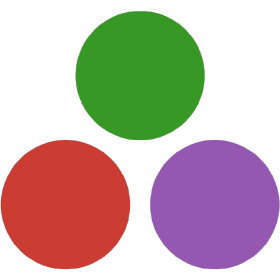
\includegraphics[height=20mm]{images/julia logo 2}};
    \end{tikzpicture}

  \begin{abstract}
    Special functions serve a unique purpose in many applications by abstracting otherwise complicated series or equations and allow for careful manipulation through utilizing their well studied properties. 
    Having numerically and computationally stable implementations is important for clear and intuitive abstraction of the functions.
    The compatibility of the implementations with the surrounding environment's methods and tools is also necessary to ensure coherence.
    Our work will cover the \href{https://github.com/JuliaMath/SpecialFunctions.jl}{\textbf{SpecialFunctions.jl}} and the \href{https://github.com/JuliaMath/HypergeometricFunctions.jl/issues}{\textbf{HyperGeometricFunctions.jl}} Julia libraries which provide implementations/interfaces for special functions and hypergeometric functions.
    We will work on Julia implementations for the error function and it's variants (erf, erfc, erfcx, erfi, Dawson, Fadeeva), which currently use wrapper function calls to external libraries,  as well as a Julia implementation for 2 kinds of the Appell hypergeometric function, which lack implementations in most programming languages.
  \end{abstract}
  \section*{Introduction}
    \subsection*{About me 
      \href{https://github.com/AhmedYKadah}{\faGithub}    
      \href{https://linkedin.com/in/ahmed-yasser-kadah-83687b269}{\faLinkedin}    
      \href{mailto:ahmadyassermo@gmail.com}{\faEnvelope[regular]}    
    }\label{sub:About} 
    Name: Ahmed Yasser Kadah
    \\Github: \href{https://github.com/AhmedYKadah}{AhmedYKadah}
    \\Email: \href{mailto:ahmadyassermo@gmail.com}{ahmadyassermo@gmail.com}    
    \\Project duration: 175 hours (Medium)

    \medskip
      \noindent Hi there! I am Ahmed Yasser Kadah, a third year Communications and Information Engineering student at the University of Science and Technology in Zewail City, Giza, Egypt.
      I recently took an advanced course in partial differential equations and special functions, so when I saw this project I thought it would be interesting to follow along this path and study the topics further when it comes to real world applications and make something that would genuinely benefit others. 
      This is my first time contributing to an open source project and just recently made my first contribution with a \href{https://github.com/JuliaMath/SpecialFunctions.jl/pull/491}{\textbf{pull request}} for a Julia implementation of the Float64 erf(x) (will be explained later). 





    \subsection*{Background on Special Functions}\label{sub:Background } % (fold)
    Special functions are a class of mathematical functions that arise in the solutions of complex physical, engineering, and mathematical problems.\cite{sf book, special functions}
   These functions are typically defined by specific properties or satisfy particular differential equations, and they include some of the most well-known functions in mathematics, such as the error function, Gamma function, and Bessel functions.

   \medskip
   This class of functions serves a unique purpose in many different applications, as they have properties which can be utilized to solve highly complex problems which otherwise have no analytic solutions, or even assist in numerical computation.

   \medskip
   Another interesting class of functions, referred to as functions of the hypergeometric type, are generalized functions, of which special functions and elementary functions are special cases.\cite{sf book, hypergeometric functions} 
   These functions also have uses in solving highly advanced problems in physics and mathematical analysis.

   \medskip
   The \href{https://github.com/JuliaMath/SpecialFunctions.jl/blob/master/src/erf.jl}{\textbf{Error Function}}, defined as $\operatorname{erf } (x)=\frac{2 }{\sqrt{\pi } }\int_{0}^{x} e ^{-t^2}\text{d}t$. 
   To those with some background in statistics, this integral would look very familiar as it is identical to the integral of a normalized gaussian distribution, scaled by a factor of 2. 
   This function is of high importance in many fields due to it's relation to the gaussian distribution and all applications which rely on the central limit theorem. 
   
   \medskip
   The \href{https://en.wikipedia.org/wiki/Appell_series}{\textbf{Appell Hypergeometric Functions}} are a set of four series which generalize the Gaussian hypergeometric series. 
   They constitute solutions to a set of defined partial differential equations, and have applications in solving problems in both pure and applied mathematics. 
   Some of these applications include those in quantum field theory, particularly in the evaluation of some Feynman integrals. \cite{appell app}


    % subsection* Background  (end)
   \subsection*{Benefits to Community}\label{sub:Benefits to Community} % (fold)
   
   Due to the nature and importance of this topic in many applications, there already exists a large number of implementations of special functions (including the error functions and it's variants) in other languages such as Wolfram Mathematica \cite{wolfram special functions, wolfram hypergeometric}, MATLAB \cite{matlab special functions, matlab hypergeometric}, Python \cite{scipy, mpmath}, C \cite{mpfr, gsl, gnu clib, cephes, ARM, amos, toms}, and others.
   This significance shows that a natural progression would be to implement Julia versions of these functions. 
   This, however, is not the only reason.

   \medskip
   \href{https://github.com/JuliaMath/SpecialFunctions.jl}{\textbf{SpecialFunctions.jl}} and \href{https://github.com/JuliaMath/HypergeometricFunctions.jl/issues}{\textbf{HyperGeometricFunctions.jl}} are Julia libraries which aim to provide Julia implementations/interfaces for special functions and hypergeometric functions.
   SpecialFunctions.jl makes use of external libraries like openlibm, openspecfun, and mpfr through wrapper functions.
   Meanwhile, HyperGeometricFunctions.jl is purely implemented in julia with several papers cited for the numerical approaches used in the implementations.

   \medskip
   One of the things that make this project of interest for a language like Julia is the full compatibility of AutoDiff methods with Julia native functions.
   Automatic differentiation (AutoDiff) is an approach to evaluating the derivative of a function through the use of techniques which automate the evaluation of partial derivates of the elementary arithmetic operations and functions through the repeated usage of the chain rule.\cite{autodiff, ForwardDiff.jl}
   In other words, if a function has an algorithm implemented in julia, AutoDiff can "trace" the code to find the elementary operations and implement it's methods. 
   This isn't the case, however, for wrapper functions for example using "ccall" (a call to a C function). 
   Since all Julia would see is the function call, the derivative for this call would need to be manually defined to be used.
   By implementing functions in julia, AutoDiff will automatically be compatible.

   \medskip
   Further, as we will see later on, the Appell functions have very few implementations. 
   Many languages only have implementations of the Appell function of the first kind $F_1$. 
   The only languages according to our findings which have implementation of all the Appell functions are Python in the mpmath\cite{mpmath hypergeometric} library and Wolfram\cite{wolfram hypergeometric}.

    
   % subsection Benefits to Community (end)
    \subsection*{Goals}\label{sub:Goals} % (fold)
      The goals of the project are to \begin{enumerate}
        \item Implement all variants of the error function in Julia
        \item Implement the Appell hypergeometric functions in Julia. 
      \end{enumerate}  

   % \medskip
      The two repositories of interest are SpecialFunctions.jl and HypergeometricFunctions.jl. 

   \medskip
      With regards to SpecialFunctions.jl, there are a few points of interest: \begin{itemize}
        \item SpecialFunctions.jl/bessel.jl and SpecialFunctions.jl/gamma.jl would appear to need julia implementations, however they are both already implemented in \href{https://github.com/JuliaMath/Bessels.jl/tree/master}{\textbf{Bessels.jl}} 
        \item All BigFloat implementations make use of the MPFR library \cite{mpfr}, but quality of execution is high and there would be no merit behind implementing Julia versions considering the difficulty of implementation
        \item The majority of the function implementations in SpecialFunctions.jl/erf.jl (the error function variants source code file) use wrapper function calls to the C standard math library \cite{gnu clib} so this will be one of our main focuses
      \end{itemize}

      With regards to HypergeometricFunctions.jl, there are a few points of interest: \begin{itemize}
        \item Function implementations are already Julia implementations
        \item It lacks implementations for the Appell functions, so this will be our main focus
      \end{itemize}

      The standard approaches for implementing special functions tend to make use of different methods of numerical approximation methods like polynomial/rational approximation. 
      In particular, an algorithm of high significance is the \href{https://en.wikipedia.org/wiki/Remez_algorithm}{\textbf{Remez algorithm}}.
      Some of the important tools which utilize this algorithm include: \begin{enumerate}
        \item \href{https://github.com/simonbyrne/Remez.jl}{\textbf{Remez.jl}}, a Julia library for constructing minimax polynomials and rational functions 
        \item \href{https://www.sollya.org/}{\textbf{Sollya}}, another powerful tool for constructing polynomials but with a less convenient interface. Will be used as the reference for the performance of Remez.jl since it is still being developed.
      \end{enumerate}
      Some of the standard approaches for implementing hypergeometric functions are Taylor and asymptotic series computations, Gauss–Jacobi quadrature, numerical solution of differential equations, recurrence relations, and others.\cite{nmhg}
      So, a lot of effort needs to be put into researching the appropriate approach for an implementation of the Appell functions.
      To best approach these implementations, researchers of interest will be contacted to give their guidance or support.
    
    \medskip
    \textit{Expected difficulties and risks:} 
    Part of this project will involve an in-depth literature review to find appropriate methods of computing these special functions and the quality and extent of documentation of existing methods will affect the speed of progress.
    % subsection* Literature Review (end)
  \newpage
  \section*{Deliverables and Timeline}\label{sec:Methods} % (fold)
    \subsection*{Deliverables}
      \begin{itemize}
        \item Full implementation of the \href{https://github.com/JuliaMath/SpecialFunctions.jl/blob/master/src/erf.jl}{\textbf{Error Function}} and it's varieties \cite{error function}
          \begin{itemize}
            \item Error Function: $\operatorname{erf } (x)=\frac{2 }{\sqrt{\pi } }\int_{0}^{x} e ^{-t^2}\text{d}t$ for Float32 and Float64 (Float64 for real values has been implemented as said previously), for real as well as complex inputs.
            \item Complementary Error Function: $\operatorname{erfc } (x)=1- \frac{2 }{\sqrt{\pi } }\int_{0}^{x} e ^{-t^2}\text{d}t$ for Float32, and Float64, for real as well as complex inputs.
            \item Scaled Complementary Error Function: $\operatorname{erfcx } (x)=e ^{x^2 } \operatorname{erfc} (x)$ for Float32, and Float64, for real as well as complex inputs.
            \item Imaginary Error Function: $\operatorname{erfi } (x)= -i \operatorname{erf} (ix)$ for Float32, and Float64, for real as well as complex inputs.
            \item Dawson Function: $D (x)=\frac{\sqrt{\pi } }{2 }e ^{-x^2 } \operatorname{erfi} (x)$ for Float32, and Float64, for real as well as complex inputs.
            \item Faddeeva Function: $w (z)=e ^{-z^2 } \operatorname{erfi} (z)= \operatorname{erfcx}(-iz)$ for Float32, and Float64, for complex inputs.
          \end{itemize}
        % \item Implementation of \href{https://github.com/JuliaMath/SpecialFunctions.jl/blob/master/src/gamma.jl}{gamma function} for real and complex inputs. 
        % \item At least 15 issues resolved on \href{https://github.com/JuliaMath/SpecialFunctions.jl/issues}{\textbf{SpecialFunctions.jl}}, which will be filtered for quality
        % \item At least 5 issues resolved on \href{https://github.com/JuliaMath/HypergeometricFunctions.jl/issues}{\textbf{HyperGeometricFunctions.jl}}, which will be filtered for quality
        % \item Documentation of previous implementation attempts and possible gaps for future work and implementations outside project scope.
        \item Full implementation of two of the \href{https://en.wikipedia.org/wiki/Appell_series}{\textbf{Appell Hypergeometric Functions}} \cite{appell, nist appell, mhs asb} 
          \begin{itemize}
            \item $F_1 $ is defined for $\lvert x  \rvert <1 $, $\lvert y  \rvert < 1 $ by the series \[
              F_1(a,b_1,b_2;c;x,y)=\displaystyle\sum_{m,n=0 }^{\infty } \displaystyle\frac{(a)_{m+n }(b_1)_{m }(b_2)_{n }}{(c)_{m+n}m!n! }x ^m y^n 
            \] 
              where $(q)_n $, the Pochhammer symbol, is defined as \[
                (x)_0=1\] \[
                (x)_n = \underbrace{x(x+1)(x+2)\dots(x+n-1)}_{n\text{ factors}}
                = \displaystyle\frac{\Gamma (x+n)}{\Gamma(x)}
              \] 
            \item $F_2 $ is defined for $\lvert x  \rvert +\lvert y  \rvert < 1 $ by the series \[
              F_2(a,b_1,b_2;c_1,c_2;x,y)=\displaystyle\sum_{m,n=0 }^{\infty } \displaystyle\frac{(a)_{m+n }(b_1)_{m }(b_2)_{n }}{(c_1)_{m}(c_2)_{n}m!n! }x ^m y^n 
            \] 
            \item (Optional) $F_3 $ is defined for $\lvert x  \rvert <1 $, $\lvert y  \rvert < 1 $ by the series \[
              F_3(a_1,a_2,b_1,b_2;c;x,y)=\displaystyle\sum_{m,n=0 }^{\infty } \displaystyle\frac{(a_1)_{m}(a_2)_{n}(b_1)_{m }(b_2)_{n }}{(c)_{m+n}m!n! }x ^m y^n 
            \] 
            \item (Optional) $F_4 $ is defined for $\lvert x  \rvert ^{1/2} +\lvert y  \rvert ^{1/2}< 1 $ by the series \[
              F_4(a,b;c_1,c_2;x,y)=\displaystyle\sum_{m,n=0 }^{\infty } \displaystyle\frac{(a)_{m+n }(b)_{m+n }}{(c_1)_{m}(c_2)_{n}m!n! }x ^m y^n 
            \] 
          \end{itemize}
      \end{itemize}
    \newpage
    \subsection*{Timeline}
      Estimated total time spent $\approx 175 $ hours 

      \noindent Average time per week $\approx 15 $ hours 
      \begin{releaseyear}{June '25}{cyan}
        \begin{releasequarter}{W 1}{cyan!50}
          \release{Literature review on polynomial and rational approximations}{$\approx 12$  hours}
          \release{$\operatorname{erf}(x)$ for real values for Float32 }{$\approx 6$  hours}
        \end{releasequarter}
        \begin{releasequarter}{W 2}{cyan!50}
          \release{$\operatorname{erfc}(x)$ for real values for Float32, and Float64}{$\approx 6$  hours}
          \release{$\operatorname{erfi}(x)$ for real values for Float 32, Float 64}{$\approx 6$  hours}
          \release{Literature review on evaluation of complex input special functions}{$\approx 8$  hours}

        \end{releasequarter}
        \begin{releasequarter}{W 3}{cyan!50}
          \release{$\operatorname{erfi}(x)$ for complex values for Float 32, Float 64}{$\approx 12$  hours}
          \release{$\operatorname{erf}(x)$ for complex values for Float 32, Float 64}{$\approx 1$  hours}
        \end{releasequarter}
        \begin{releasequarter}{W 4}{cyan!50}
          \release{$\operatorname{erfc}(x)$ for complex values for Float 32, Float 64}{$\approx 12$  hours}
        \end{releasequarter}
      \end{releaseyear}
      \begin{releaseyear}{July '25}{teal}
        \begin{releasequarter}{W 1}{teal!50}
          \release{$\operatorname{erfcx}(x)$ for real values for Float 32, Float 64}{$\approx 6$  hours}
          \release{$\operatorname{erfcx }(x)$ for complex values for Float 32, Float 64}{$\approx 12$  hours}
        \end{releasequarter}
        \begin{releasequarter}{W 2}{teal!50}
          % \release{Prepare for midterm evaluation}{}
          \release{$D(x)$ for real values for Float 32, Float 64}{$\approx 6$  hours}
          \release{$D(x)$ for complex values for Float 32, Float 64}{$\approx 12$  hours}
        \end{releasequarter}
        \begin{releasequarter}{W 3}{teal!50}
          \release{Literature review on methods of evaluating Appell functions}{$\approx 6$  hours}
          \release{$w(x)$ for complex values for Float 32, Float 64}{$\approx 12$  hours}
          \release{\textbf{Midterm Evaluation}}{}
        \end{releasequarter}
        \begin{releasequarter}{W 4}{teal!50}
          \release{First Appell function}{$\approx 16$  hours}
        \end{releasequarter}
      \end{releaseyear}
      \begin{releaseyear}{August '25}{orange}
        \begin{releasequarter}{W 1}{orange!50}
          \release{First Appell function}{$\approx 16$  hours}
        \end{releasequarter}
        \begin{releasequarter}{W 2}{orange!50}
          \release{Second Appell function}{$\approx 16$  hours}
        \end{releasequarter}
        \begin{releasequarter}{W 3}{orange!50}
          \release{Second Appell function}{$\approx 16$  hours}
        \end{releasequarter}
        \begin{releasequarter}{W 4}{orange!50}
          \release{\textbf{Final week}}{}
        \end{releasequarter}
      \end{releaseyear}


      % \vspace{5px}

  
  % section* Methods (end)
  \section*{Related Work}\label{sec:Results} % (fold)
  \subsection*{Special Functions}\label{sub:Special Functions} % (fold)
  % subsection Hypergeometric Functions (end)
   Most notable languages have some form of implementation of the error function and most/all of its varients because it is simply too important to leave out.
   There are also various C math libraries with Julia interfaces which include special function calls like GSL, openlibm, and openspecfun.

  
  % subsection Special Functions (end)

  \subsection*{Hypergeometric Functions}\label{sub:Hypergeometric Functions} % (fold)
    The resources for hypergeometric are a bit less available than special functions. 
    Implementations for the Appell functions are somewhat rare, and mostly restricted to the first kind $F_1$.
    % Considering the language of interest: 
    % MATLAB lacks built in implementations for any of the Appell functions, and the user implementations are poor quality.
    Wolfram is likely the only language which has all Appell functions built in.
    Also, python's mpmath library (open source and available for use under BSD license) does have all the variant and could be used as a reference.
  
  % % section* References (end)
  % \section*{References}\label{sec:References} % (fold)
    
    \begin{thebibliography}{9}
      \bibitem{sf book}
      Larry C. Andrews, \textit{"Special Functions of Mathematics for Engineers"}, 2nd Edition

      \bibitem{special functions}
      Special Functions \url{https://en.wikipedia.org/wiki/Special_functions}  

      \bibitem{hypergeometric functions}
      Hypergeometric Functions \url{https://en.wikipedia.org/wiki/Hypergeometric_function}

      \bibitem{wolfram special functions}
      Wolfram list of special functions \url{https://reference.wolfram.com/language/guide/SpecialFunctions.html.en}

      \bibitem{wolfram hypergeometric}
      Wolfram list of hypergeometric functions \url{https://reference.wolfram.com/language/guide/HypergeometricFunctions.html}

      \bibitem{matlab special functions}
      MATLAB list of special functions \url{https://www.mathworks.com/help/matlab/special-functions.html}

      \bibitem{matlab hypergeometric}
      MATLAB list of hypergeometric functions \url{https://www.mathworks.com/help/symbolic/sym.hypergeom.html}

      \bibitem{scipy}
      {{SciPy}: Fundamental Algorithms for Scientific Computing in Python} \url{https://docs.scipy.org/doc/scipy/reference/special.html}

      \bibitem{mpmath}
      mpmath: a {P}ython library for arbitrary-precision floating-point arithmetic \url{https://mpmath.org/}
      
      \bibitem{mpmath hypergeometric}
      mpmath list of hypergeometric functions \url{https://mpmath.org/doc/current/functions/hypergeometric.html}

      \bibitem{mpfr}
      MPFR: a C library for multiple-precision floating-point computations with correct rounding \url{https://www.mpfr.org/}

      \bibitem{gsl}
      GNU Scientific Library \url{https://www.gnu.org/software/gsl/}

      \bibitem{gnu clib}
      The GNU Standard C library \url{https://sourceware.org/git/?p=glibc.git}

      \bibitem{cephes}
      Cephes Mathematical Library \url{https://www.netlib.org/cephes/}

      \bibitem{ARM}
      ARM Optimized Routines \url{https://github.com/ARM-software/optimized-routines/tree/master/math}

      \bibitem{amos}
      AMOS A Portable Package for Bessel Functions of a Complex Argument and Nonnegative Order\url{https://www.netlib.org/amos/}

      \bibitem{toms}
       ACM Collected Algorithms \url{https://www.netlib.org/toms-2014-06-10/}

      \bibitem{autodiff}
      Automatic Differentiation \url{https://en.wikipedia.org/wiki/Automatic_differentiation}

      \bibitem{ForwardDiff.jl}
      Forward-Mode Automatic Differentiation in {J}ulia \url{https://github.com/JuliaDiff/ForwardDiff.jl}

      \bibitem{error function}
      The Error Function \url{https://en.wikipedia.org/wiki/Error_function}

      \bibitem{appell}
      The Appell Functions \url{https://en.wikipedia.org/wiki/Appell_series}

      \bibitem{appell app}

      Kim, I., \& Rathie, A. K. (2023). "\textit{A Note on Certain General Transformation Formulas for the Appell and the Horn Functions}," Symmetry, 15(3), 696. \url{https://doi.org/10.3390/sym15030696}

      
      \bibitem{SpecialFunctions.jl}
      The SpecialFunctions.jl Julia Library \url{https://github.com/JuliaMath/SpecialFunctions.jl}

      \bibitem{HypergeometricFunctions.jl}
      The HyperGeometricFunctions.jl Julia Library \url{https://github.com/JuliaMath/HypergeometricFunctions.jl}

      \bibitem{remez}
      The Remez Algorithm \url{https://en.wikipedia.org/wiki/Remez_algorithm}

      \bibitem{remez.jl}
      The Remez.jl Julia Library \url{https://github.com/simonbyrne/Remez.jl}

      \bibitem{sollya}
      Sollya: an environment for the development of numerical codes \url{https://www.sollya.org/}

      \bibitem{nist appell}
      Appell Functions, NIST \url{https://dlmf.nist.gov/16.13}

      \bibitem{mhs asb}
      Michael J. Schlosser, \textit{"Multiple Hypergeometric Series – Appell Series
      and Beyond"}, \url{https://www.mat.univie.ac.at/~schlosse/pdf/appell-survey.pdf}

      \bibitem{nmhg}
      Pearson, J.W., Olver, S. \& Porter, M.A. "\textit{Numerical methods for the computation of the confluent and Gauss hypergeometric functions}". Numer Algor 74, 821–866 (2017). \url{https://doi.org/10.1007/s11075-016-0173-0}

   \end{thebibliography}
  
  % section* References (end)
\end{document}
